
\section{Probabilistic Robotics}

Robotics, according to Thrun et al.\cite{Thrun:2005:PR:1121596}, is the science of perceiving and manipulating the physical world through computer-controlled mechanical devices and it is taking place in wide areas such as medicine\cite{Azad:STAR}, planet exploration\cite{Geoffrey:venus}, agriculture\cite{Shamshiri:research-agricultural}, construction\cite{Pileun:construction}, entertainment\cite{Morris:entertainment} among others. 

The robotics that is known nowadays has being evolved across the years. From robotic systems designed to automatize highly repetitive and physically demanding human tasks in the early-to-mid-1940s\cite{Ferreira:prob}, passing through researches making the strong assumption of having exact models of robots and environments in the 1970s, to probabilistic robotics in the mid-1990s\cite{Thrun:robotic-statistics}. Thus a robot needs to deal with uncertainty most of the time. As an example, a robot ordered to walk 1 meter forward from its current position will not end up exactly 1 meter far from its initial position due to some errors, if the robot speed was high and it slipped or the noise produced by the actuators is significant. That is why it needs to be capable to deal with uncertainty, predicting and preserving its current position and orientation within the environment\cite{Nikos:auxiliary-pf}.

\subsection{State}

State, according to Thrun et al.\cite{Thrun:2005:PR:1121596}, refers to the set of all aspects of the robot and its environment that can influence to the future. Two types of state can be defined:

\begin{itemize}
\item \textbf{Dynamic state} changes its position over time. For instance, the people or other robots location.
\item \textbf{Static state} does not change its position over time. For example, the walls or other moveless objects location.
\end{itemize}

Some instances of state are: 

\begin{itemize}
\item The position of physical static entities in the environment as walls, boxes, doors, etc.
\item The location and speed of mobile entities in the environment as people, other robots, etc.
\item The robot pose is usually defined by its position and its orientation relative to a global reference frame. A robot moves on a \textit{fixed frame} which is attached to the ground and does not move. This frame is called the \textit{global reference frame} (GRF). Additionally, a robot is linked within a frame which moves along with the robot. This frame is referred as \textit{local reference frame} (LRF). Communication between the coordinate frames is known as \textit{transformation of frames} and it is a key concept when modeling and programming a robot\cite{Reza:Theory-of-applied-robotics}. Figure \ref{fig:ch-2-global-local} illustrates the difference between GRF and LRF where the $X_R$ axis points to the right side of the robot, the $Y_R$ axis is aligned to its longitudinal axis and the $Z_R$ axis points upward. Besides to these Cartesian coordinates, the robot's angle orientation is defined by the Euler angles: Yaw, Pitch and Roll (see \cite{Cook:mobile-robots}). 
\end{itemize}

The notation used to represent a state at time $t$ will be denoted as $x_t$.

\begin{figure}[h!]
  \centering
  \begin{subfigure}[b]{0.5\linewidth}
  	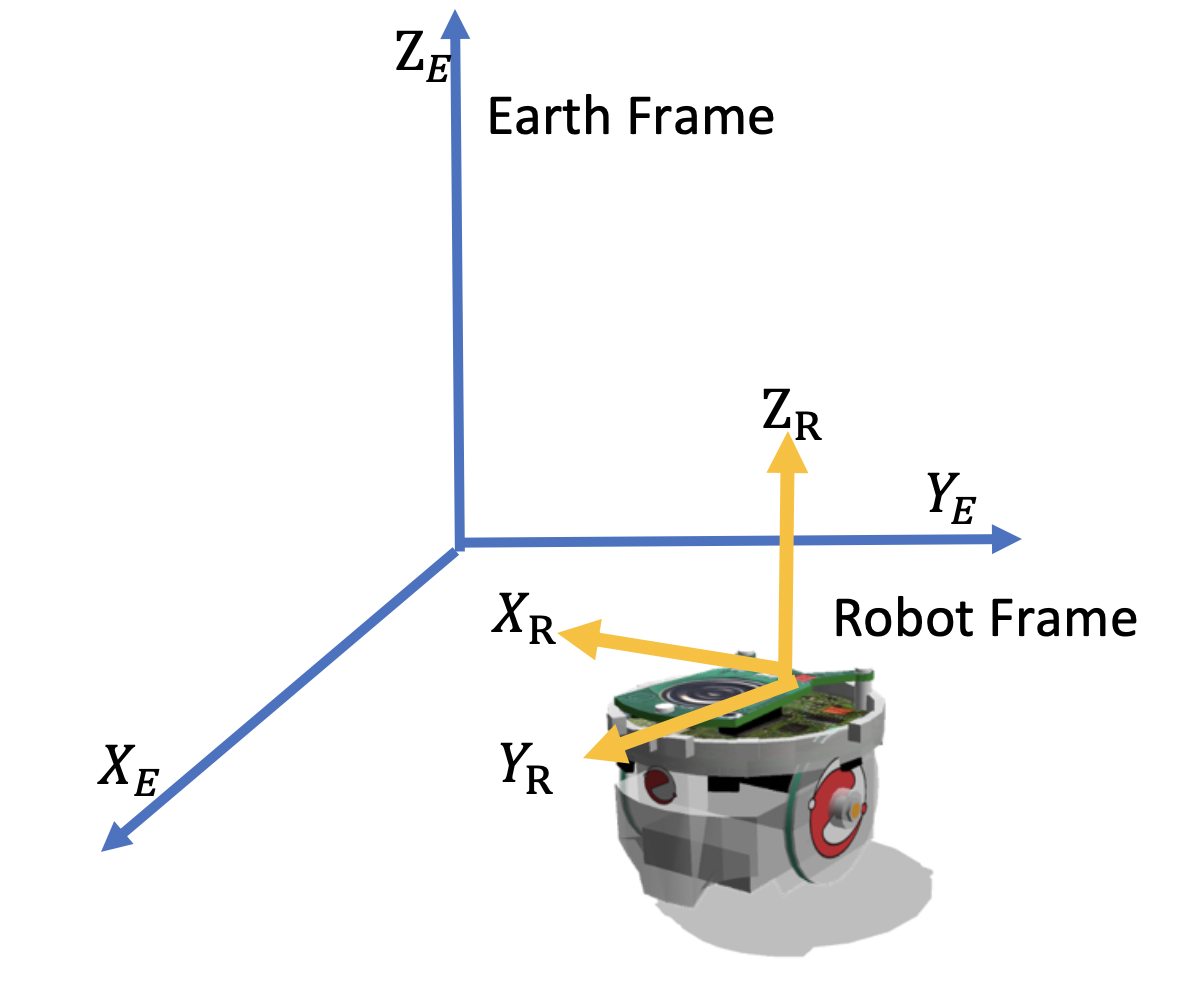
\includegraphics[width=\linewidth]{\images/chapter2/local-system.png}
  \end{subfigure}
  \caption{Local vs Global reference frame}
  \label{fig:ch-2-global-local}
\end{figure}

\subsection{Robot Versus The Environment}

A robot can interact with the environment in two ways. First, it can modify the environment state using its actuators which are drivers acting as muscles that let the robot change its configuration\cite{Reza:Theory-of-applied-robotics}. For instance, a rotational motor is an actuator that can power a joint and thus changing the robot pose. As another example, a robotic arm can be used to move objects from one position to another. Second, a robot can sense the environment using its sensors which are elements, usually attached to the robot, for obtaining information about internal and environmental states \cite{Reza:Theory-of-applied-robotics}\cite{Thrun:2005:PR:1121596}. 

The control data is information about the change of state in the environment\cite{Thrun:2005:PR:1121596}. It can be, for instance, the velocity or the acceleration of the robot at a given time $t$ and thus it will be represented as $u_t$.  The sensor data provided at time $t$ is denoted as $z_t$ and therefore a sequence of sensor observations will be $z_{1:t}= {z_1, z_2, ..., z_t}$.

\subsection{Belief Representation}\label{ch-2:sub:belief-representation}

A belief is a representation of the internal state of the robot about its position in the environment whereas the true state is where the robot truly is in the environment. In other words it is the probability that a robot at time $t$ is at location $x$ given previous sensor data $z_1, z_2, ..., z_t$ and previous control actions $u_1, u_2, ..., u_t$. A belief can be expressed as the conditional probability function of state $x_t$ given sensor data $z_{1:t} \text{ and control actions } u_{1:t}$. Thus it assigns a probability to each location in the environment, dealing with a single-hypothesis belief (robot tracks a single possible solution) or multiple-hypothesis beliefs (robot tracks an infinite set of positions)\cite{Siegwart:intro-autonumous-robots}. Following Thrun et al. notation, a belief over a state variable $x_t$ will be denoted as $bel(x_t)$ which is the posterior density conditioned on all past measurements and control actions.

\begin{equation}
bel(x_t) = p(x_t | z_{1:t}, u_{1:t})
\label{eq:ch2:bel-update}
\end{equation}

Equation \ref{eq:ch2:bel-posterior} shows the posterior without including the last measurement data. It is usually called $prediction$ in the probabilistic filtering area.

\begin{equation}
\overline{bel}(x_t) = p(x_t | z_{1:t-1}, u_{1:t})
\label{eq:ch2:bel-posterior}
\end{equation}

The probability $bel(x_t)$ can be calculated using the previous posterior belief before measurement $z_t$ and after taking action $u_t$, that is $\overline{bel}(x_t)$. This is known as correction\cite{Thrun:robotic-statistics}. 

The relation between equation \ref{eq:ch2:bel-update} and \ref{eq:ch2:bel-posterior} is shown in appendix \ref{eq:ch-2:bel-derivation}.

\subsection{The Markov Property}

The $Markov Property$ states that a future state depends on the present state only and thus it resumes all the past states information.

Formally, let $x_t$ be a stochastic discrete process that can take on a discrete set of values, where $t \in \mathbb{N}$. A value in process $x_t$ has the \textit{Markov Property} if for all $t$ such that $t\geq1$, the probability distribution of $x_{t+1}$ is determined by the state $x_t$ of the process at time $t$, and does not rely on past values $x_t$ for $t = 0, 1, ..., t - 1$\cite{Privault:markov-chains}. That is:

\begin{equation}
p(x_{t+1} | x_t, x_{t-1}, ..., x_0) = p(x_{t+1} | x_t)
\end{equation}

The Markov Property is an approximation, commonly used in mobile robotics since it simplifies tracking, reasoning and planning and hence it has been found to be very robust for such applications\cite{Siegwart:intro-autonumous-robots}. 


\subsection{Localization Methods}

Navigation is about controlling and operating the course of a robot and it is one of the most challenging skills that a mobile robot needs to master in order to successfully moving through the environment. According to Siegwart et al. what is important for a robot to succeed in navigation is to succeed likewise in these four blocks of navigation:

\begin{itemize}
\item \textit{Sense:} the robot perceives the environment though its sensors and extract meaningful data in order to process and obtain information.
\item \textit{Localization:} the robot knows where it is in the environment.
\item \textit{Cognition:} the robot creates an execution plan in how to act to reach its goals.
\item \textit{Control Action:} the robot executes the execution plan through modulating its output motors.
\end{itemize}

Sensors and actuators take part in determining the robot's localization but both are subjected to noise and thus the problem of localization becomes difficult. Another problem with sensors is that they usually does not provide enough information content to determine the position of the robot and therefore make it easy for the robot to be in an ambiguous location. This problem is known as sensor aliasing and along with sensors and actuators noise turns the localization problem into a difficult task\cite{Siegwart:intro-autonumous-robots}.

There are two types of localization methods categorized by the increased degree of difficulty as stated in Ferreira et al.\cite{Ferreira:prob}: 

\begin{itemize}
\item \textit{Local techniques} (also called position tracking\cite{Thrun:2005:PR:1121596}), when the robot knows its initial position and it is not able to recover it if the robot loses track of it.
\item \textit{Global techniques} (see also \cite{Feng:where-am-I}), when the robot does not have any information about its initial position and it is able to estimate it even in a global uncertainty. This technique includes the \textit{kidnapped robot problem} in which a robot that knows its position is kidnapped and take it into another unknown location and its task is to recover its position. According to Thrun et al.\cite{Thrun:2005:PR:1121596} the later should be categorized as a third localization technique given its difficulty. This technique is more powerful than the former because it deals with global uncertainty and consequently a robot is able to recover its position even if its error is significant.
\end{itemize}

Local techniques approximate the pose using unimodal techniques contrary to global techniques where the robot’s internal knowledge about the state of the environment is represented by a probability density function (pdf) over the space of all locations\cite{Thrun:robotic-statistics}. An example of a global technique is shown in section \ref{sec:ch-2:particles-filter} where a robot handles multiple ambiguous positions. Then after moving, it can sense other factors in the environment that can lead to disambiguate its pose and put most of the probability in a single location and therefore having a better idea of where truly is as image \ref{fig:ch-2:particles-ex} illustrates. A more extensive and explicative example can be found in \cite{Thrun:robotic-statistics} and \cite{Liao:bayesian-filters} where the global localization problem is illustrated in a one-dimension space with a robot that has an hypothetical sensor that senses the presence of doors, when the robot finds the first door, the probability is distributed to all the places where there are doors (see figure \ref{fig:ch-2:sensors}). Thus the probability to be near a door is higher when the sensor detects a door but the robot does not know at this point which door is facing. Moving the robot forward makes the sensor to sense another door and thus increasing the probability of being at the second door. This example illustrates some important properties of the Bayes Filter.

\begin{figure}[h!]
  \centering
  \begin{subfigure}[b]{\linewidth}
  	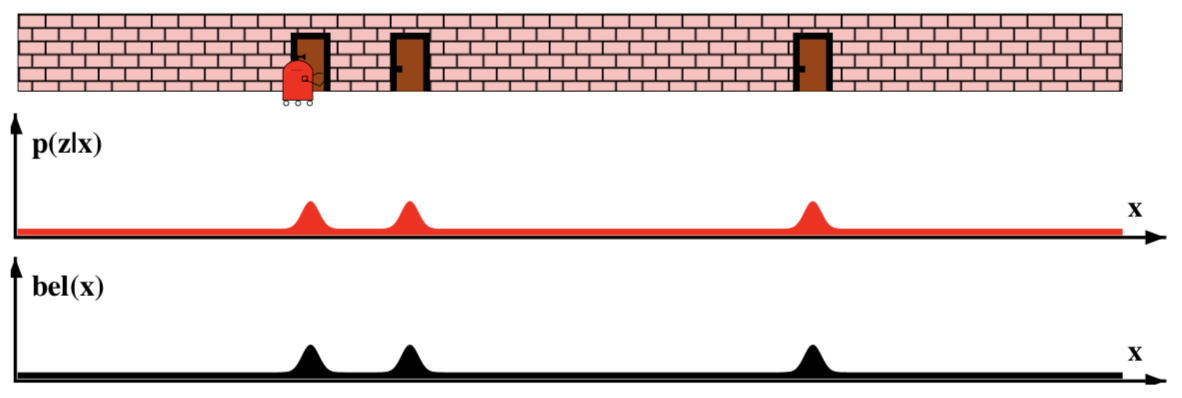
\includegraphics[width=\linewidth]{\images/chapter2/first-door.png}
  \end{subfigure}
  \vspace{1cm}
  \begin{subfigure}[b]{\linewidth}
  	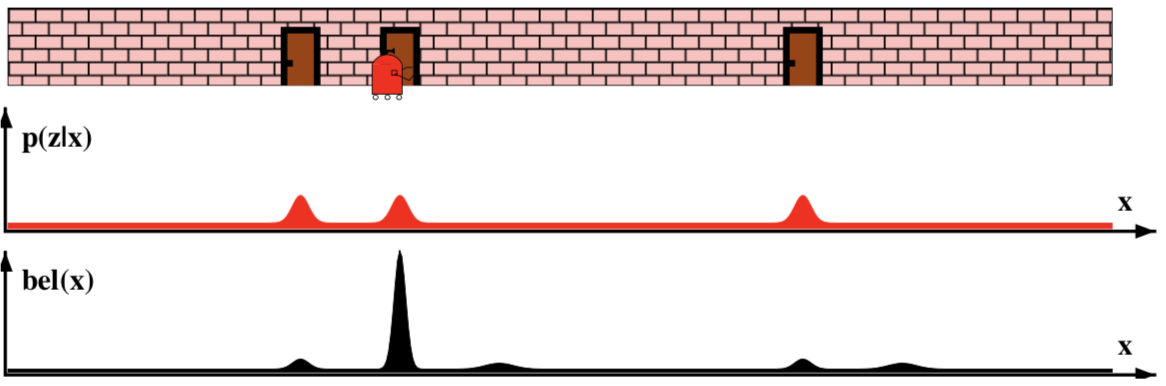
\includegraphics[width=\linewidth]{\images/chapter2/second-door.png}
  \end{subfigure}
  \caption{Probability density when robot senses.}
  \source{Extracted from Thrun et al. Probabilistic Robotics\cite{Thrun:robotic-statistics}}
  \label{fig:ch-2:bayes-filter-example}
\end{figure}


\subsection{Bayes Filter}\label{sec:ch-2:bayes-filter}

As claimed by Borriello et al.\cite{Liao:bayesian-filters} Bayes Filter is a statistically estimator of dynamic system's states based on noisy observations. In other words it is an algorithm that calculates beliefs distribution based on measurements and control data\cite{Thrun:2005:PR:1121596}. This is generally done in two steps as it was mentioned in section \ref{ch-2:sub:belief-representation}: the prediction and the correction step and thus each time a robot receives the sensors measurement data the robot controller software needs to compute the posterior densities shown in equation \ref{eq:ch2:bel-posterior} but notice that such task is computationally heavy and consequently its time complexity grows exponentially because the amount of sensors measurements increasing over time. A solution to this problem is to assume that such dynamic system has the Markovian Property. That is the future state $x_{t+1}$ depends on the present state $x_t$ because the assumption that $x_t$ carries all the needed information is made.

Bayes filter algorithm is recursive. It needs the previous posterior distribution to calculate the current posterior distribution. The algorithm is described below and its correctness is shown in appendix \ref{sec:ap:bayes-filter}.

\IncMargin{1em}
\begin{algorithm}

\SetKwInOut{Input}{input}\SetKwInOut{Output}{output}
\Input{$bel(x_{t-1})$, $u_t$, $z_t$}
\Output{$bel(x_t)$}
\BlankLine

  \ForEach{$x_t$}{
    $\overline{bel}(x_t)\leftarrow \int p(x_t | u_t, x_{t-1}) \: bel(x_{t-1}) dx_{t-1}$\\
    ${bel}(x_t)\leftarrow \eta \: p(z_t | x_t) \: \overline{bel}(x_t)$\\
  }
  \Return $bel(x_t)$
\caption{Bayes Filtering Algorithm\cite{Thrun:2005:PR:1121596}}

\label{ch-2:algo:bayes-filter}
\end{algorithm}\DecMargin{1em}

There are many algorithms that apply Bayes Filtering. Some examples are stated below.
\begin{itemize}
\item The \textit{Kalman Filter} (KF) is a Gaussian technique invented in 1950 by Rudolph Emil Kalman\cite{Kalman:filter} and was first implemented by NASA in the Apollo program to estimate the trajectory of the space capsule in real time\cite{Barrau:IKF}. It takes noisy data and put the noise apart in order to get information with less uncertainty\cite{Matthew:kalman-tutorial}. It works with continuous states and it represents the beliefs by the first and second moment\cite{Liao:bayesian-filters} from multivariate normal distributions. Chen et al. have proposed another version of KF called Maximum Correntropy Kalman Filter (MCKF) which is an effective and robust algorithm for non-Gaussian signals and heavy-tailed impulsive noise. Instead of using the Minimum Mean Square Error (MMSE) as KF, its optimality criterion is the Maximum Correntropy Criterion (MCC)\cite{Chen:MCKF}. 
\item The \textit{Extended Kalman Filter} (EKF) does not assume any linearity as KF does and thus the next state and the measurement probabilities are nonlinear functions\cite{Zarchan:fundam-kalman}\cite{Thrun:2005:PR:1121596}. Some variants of this method include Unscented Kalman Filter, where the state distribution is approximated by a Gaussian random variable as in EKF, but now a minimal set of sample points are cautiously chosen for representing the state distribution\cite{Julier:UKF}\cite{Wan:UKF}. Another improvement of EKF is the Invariant Extended Kalman Filter (IEKF) used for continuous-time systems with discrete observations\cite{Barrau:IEKF}.
\item The \textit{Grid-based Filters} split the environment into small grids, each containing a belief of the true position state\cite{Liao:bayesian-filters}. For instance, Burgard et al. proposed a bayesian approach based on certainty grids where each cell has associated a probability of the robot to be on that cell and thus they successfully predicted the robot absolute position and orientation in a global localization problem using standard sensors in complex environments\cite{Burgard:grid-based}.
\item \textit{Topological} approaches represent the environment using graphs where each node is a representation of a location and the edges are the connectivity between two locations\cite{Liao:bayesian-filters}.
\item The \textit{Particles Filter} (PF) according to Rekleitis, uses many copies of the variable of interest, each of them is associated with a weight representing the quality of that specific particle. Each particle executes the same control action plus some noise, they are reevaluated, its weight is recalculated and therefore the particles with low weight are eliminated in a process called resampling\cite{Rekleitis:particles-filter}.
\end{itemize}

\subsection{Particles Filter}\label{sec:ch-2:particles-filter}

Particles Filter is a nonparametric implementation of the Bayes Filter algorithm where the posterior is approximated by a set of $M$ samples called \textit{particles} where $M$ is usually a large number(e.g. 2000). Under the context of localization, it is also known as Monte Carlo localization (MCL)\cite{Thrun00j}. Each particle has associated a weight that represents the contribution to the overall estimate of the posterior\cite{Rekleitis:particles-filter}. Thus equation \ref{eq:ch-2:particles}  shows the believe at time $t$ approximated by a set of particles and weights of $M$ particles.

\begin{equation}\label{eq:ch-2:particles}
bel(x_t) \approx S_t = \lbrace \langle x_t^{[m]},w_t^{[m]} \rangle |  1 \leq m \leq M \rbrace
\end{equation}

Where $x$ denotes the state of particle $m$, and $w$ represents the weight of such particle. 

According to Thrun et al. the probability of including a particle $x_t^{[m]}$ will be proportional to its posterior belief (see equation \ref{eq:ch-2:particles-proportion}) and thus more particles in a region of the environment means that the true state is more likely to be in that region.

\begin{equation}\label{eq:ch-2:particles-proportion}
x_t^{[m]} \sim p(x_t | z_{1:t}, u_{1:t})
\end{equation}

Table \ref{ch-2:algo:particles-filter} illustrates the Particles Filter algorithm. The algorithm has two loops, representing the prediction and resampling steps respectively. The prediction step obtains M hypothesis about the true state using sampling techniques. All of these hypothesis together correspond to $\overline{bel}(x_t)$ in the Bayes algorithm. Furthermore the weight or importance factor for each particle is calculated as a conditional probability of sensing $z_t$ given the state of that specific particle representing the posterior $bel(x_t)$ in the Bayes algorithm. The resampling step consists in selecting with replacement M particles from the temporal data set $\bar{S_t}$ with probability proportional to each particles' weight and thus the particles with lower weights have less probability to be selected\cite{Thrun:2005:PR:1121596}. Figure \ref{fig:ch-2:particles-ex} illustrates the use of MCL for robot localization.

\IncMargin{1em}
\begin{algorithm}

\SetKwInOut{Input}{input}\SetKwInOut{Output}{output}
\Input{$S_{t-1}$, $u_t$, $z_t$}
\Output{$S_t$}
\BlankLine
$\bar{S_t} \leftarrow \emptyset$\\
$S_t \leftarrow \emptyset$\\
  \For{$m = 1$ to $M$}{
    sample $x_t^{[m]}\backsim p(x_t | u_t, x_{t-1}^{[m]})$ \\
    $w_t^{[m]} \leftarrow p(z_t | x_t^{[m]}) $\\
    $\bar{S_t} \leftarrow \bar{S_t} \cup \lbrace \langle x_t^{[m]},w_t^{[m]} \rangle \rbrace$\\
  }
  \For{$m = 1$ to $M$}{
    $\langle x_t, w_t \rangle \leftarrow \text{draw } i \text{ from } \bar{S_t} \text{ with probability } \propto w_t^{[i]}$\\
    ${S_t} \leftarrow {S_t} \cup \lbrace \langle x_t, w_t \rangle \rbrace$\\
  }
  \Return $S_t$
\caption{Particles Filtering Algorithm. Adapted from \cite{Thrun:2005:PR:1121596}.}

\label{ch-2:algo:particles-filter}
\end{algorithm}\DecMargin{1em}

Rekleitis et al. mention other resampling techniques: Linear Time Resampling and Resampling by Liu et al. The former uses the method of simulating order statistics\cite{Gerontidis:stats}, that is, obtaining $M+1$ random numbers, applying the negative log number and then calculating their cumulative sum, then compare them to the cumulative sum over the weights in order to generate a list of indexes corresponding to the particles with higher weights\cite{Carpenter:improved-pf}. Resampling by Liu et al. proposed the use of a function of the weights ($a_j=f(w_j)$), for instance the square root $f(w_j) = \sqrt w_j$ and then normalize this quantity regarding the number of particles M. Then if $a_j$ is greater or equal to one, the $jth$ particle is duplicated $k$ times, where $k=\lfloor a_j \rfloor$; otherwise the particle is selected with a probability equal to $a_j$\cite{Liu:resampling}\cite{Rekleitis:particles-filter}.

Zhou et al. proposed an improved PF algorithm called the Pearson Particles Filter (PPF) because it is based on the Pearson Correlation Coefficient (PCC) which is a statistical technique to determine the linear dependence between two random variables and thus it is used to decide how close the hypothetical particle state is to the true state value. Even though this technique solves the degeneracy and sample impoverishment problem present in PF, it is computationally complex\cite{Zhou:sampling-method}. 

Murray et al. present an alternative to accelerate the resampling technique eliminating the cumulative sum over weights using two schemes based on Metropolis\cite{Metropolis:fast-computing} and rejection samplers making the problem of resampling parallelizable using graphical processing units (GPU)\cite{Murray:parallel-res}. Nicely et al. go even further, introducing a general purpose graphical processing units (GPGPUs) implementation which takes advantage of the properties of the cumulative sum and the evolutionary nature of the particle weighting process to parallelize the re-index section of the algorithm\cite{Nicely:improvised-parallel-res}.


\begin{figure}[h!]
  \centering
  \begin{subfigure}[b]{0.65\linewidth}
  	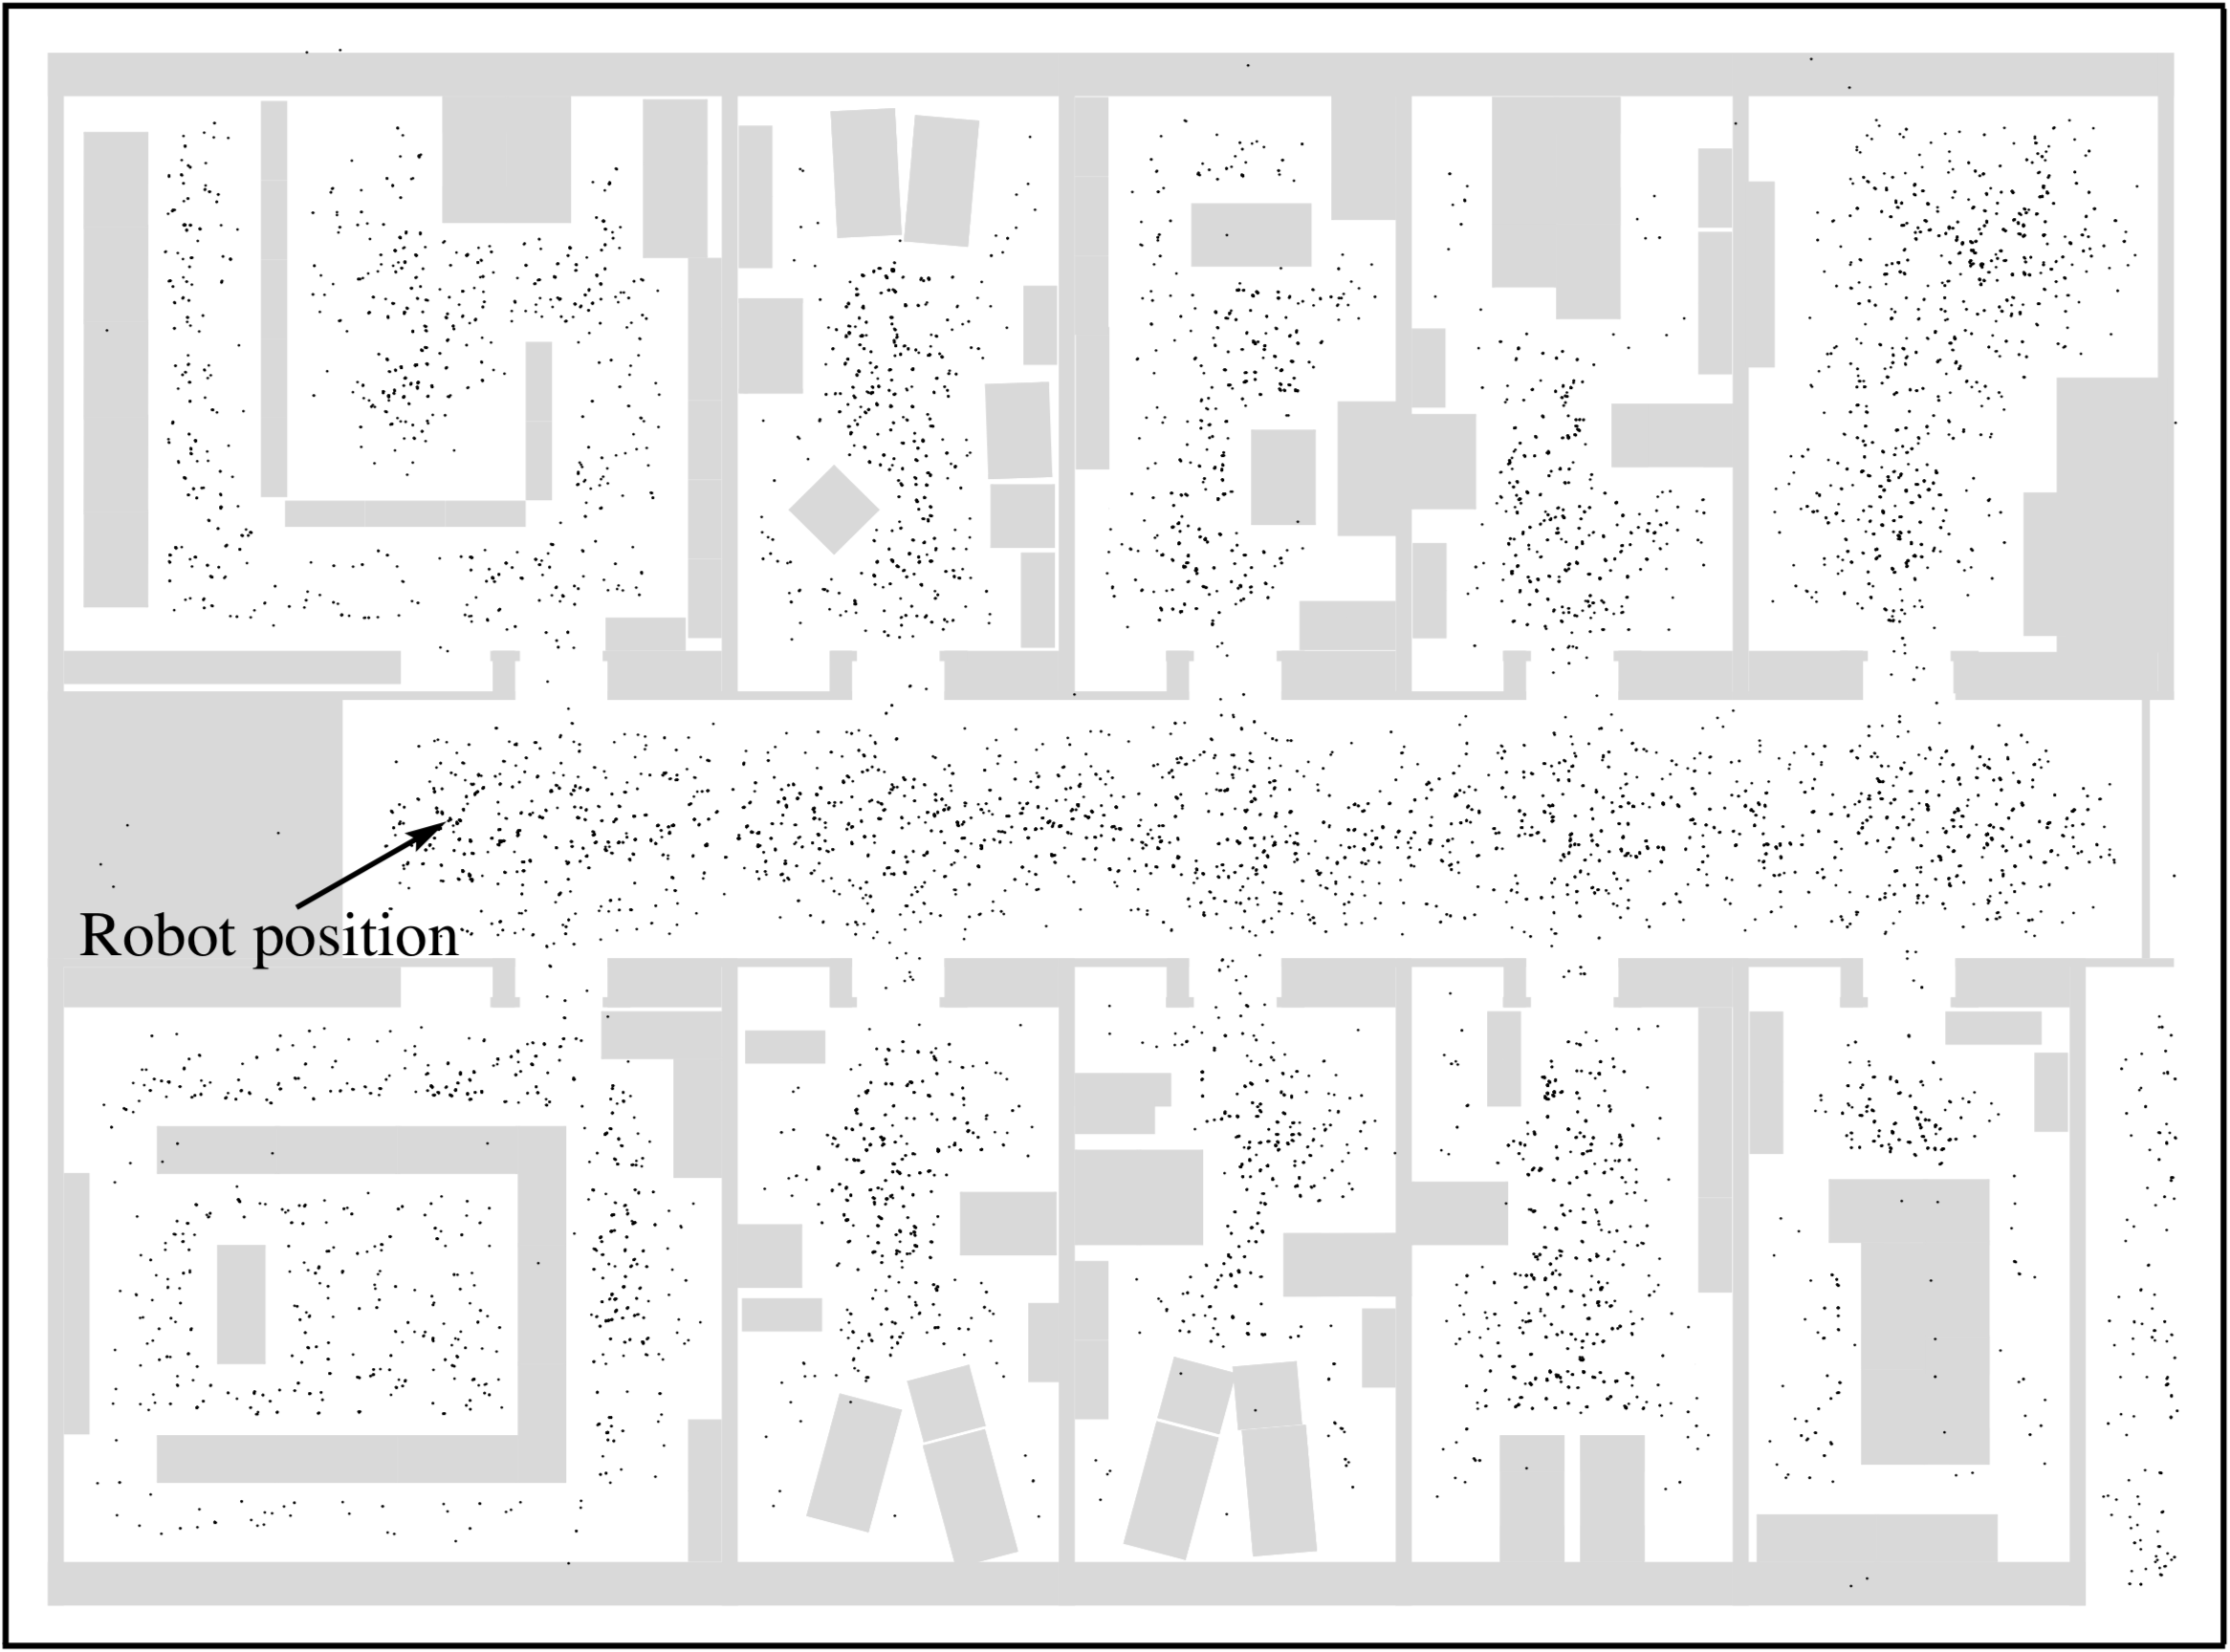
\includegraphics[width=\linewidth]{\images/chapter2/particles-1.png}
	\caption{}
  	\label{fig:ch-2:particles-1}
  \end{subfigure}
  \begin{subfigure}[b]{0.47\linewidth}
  	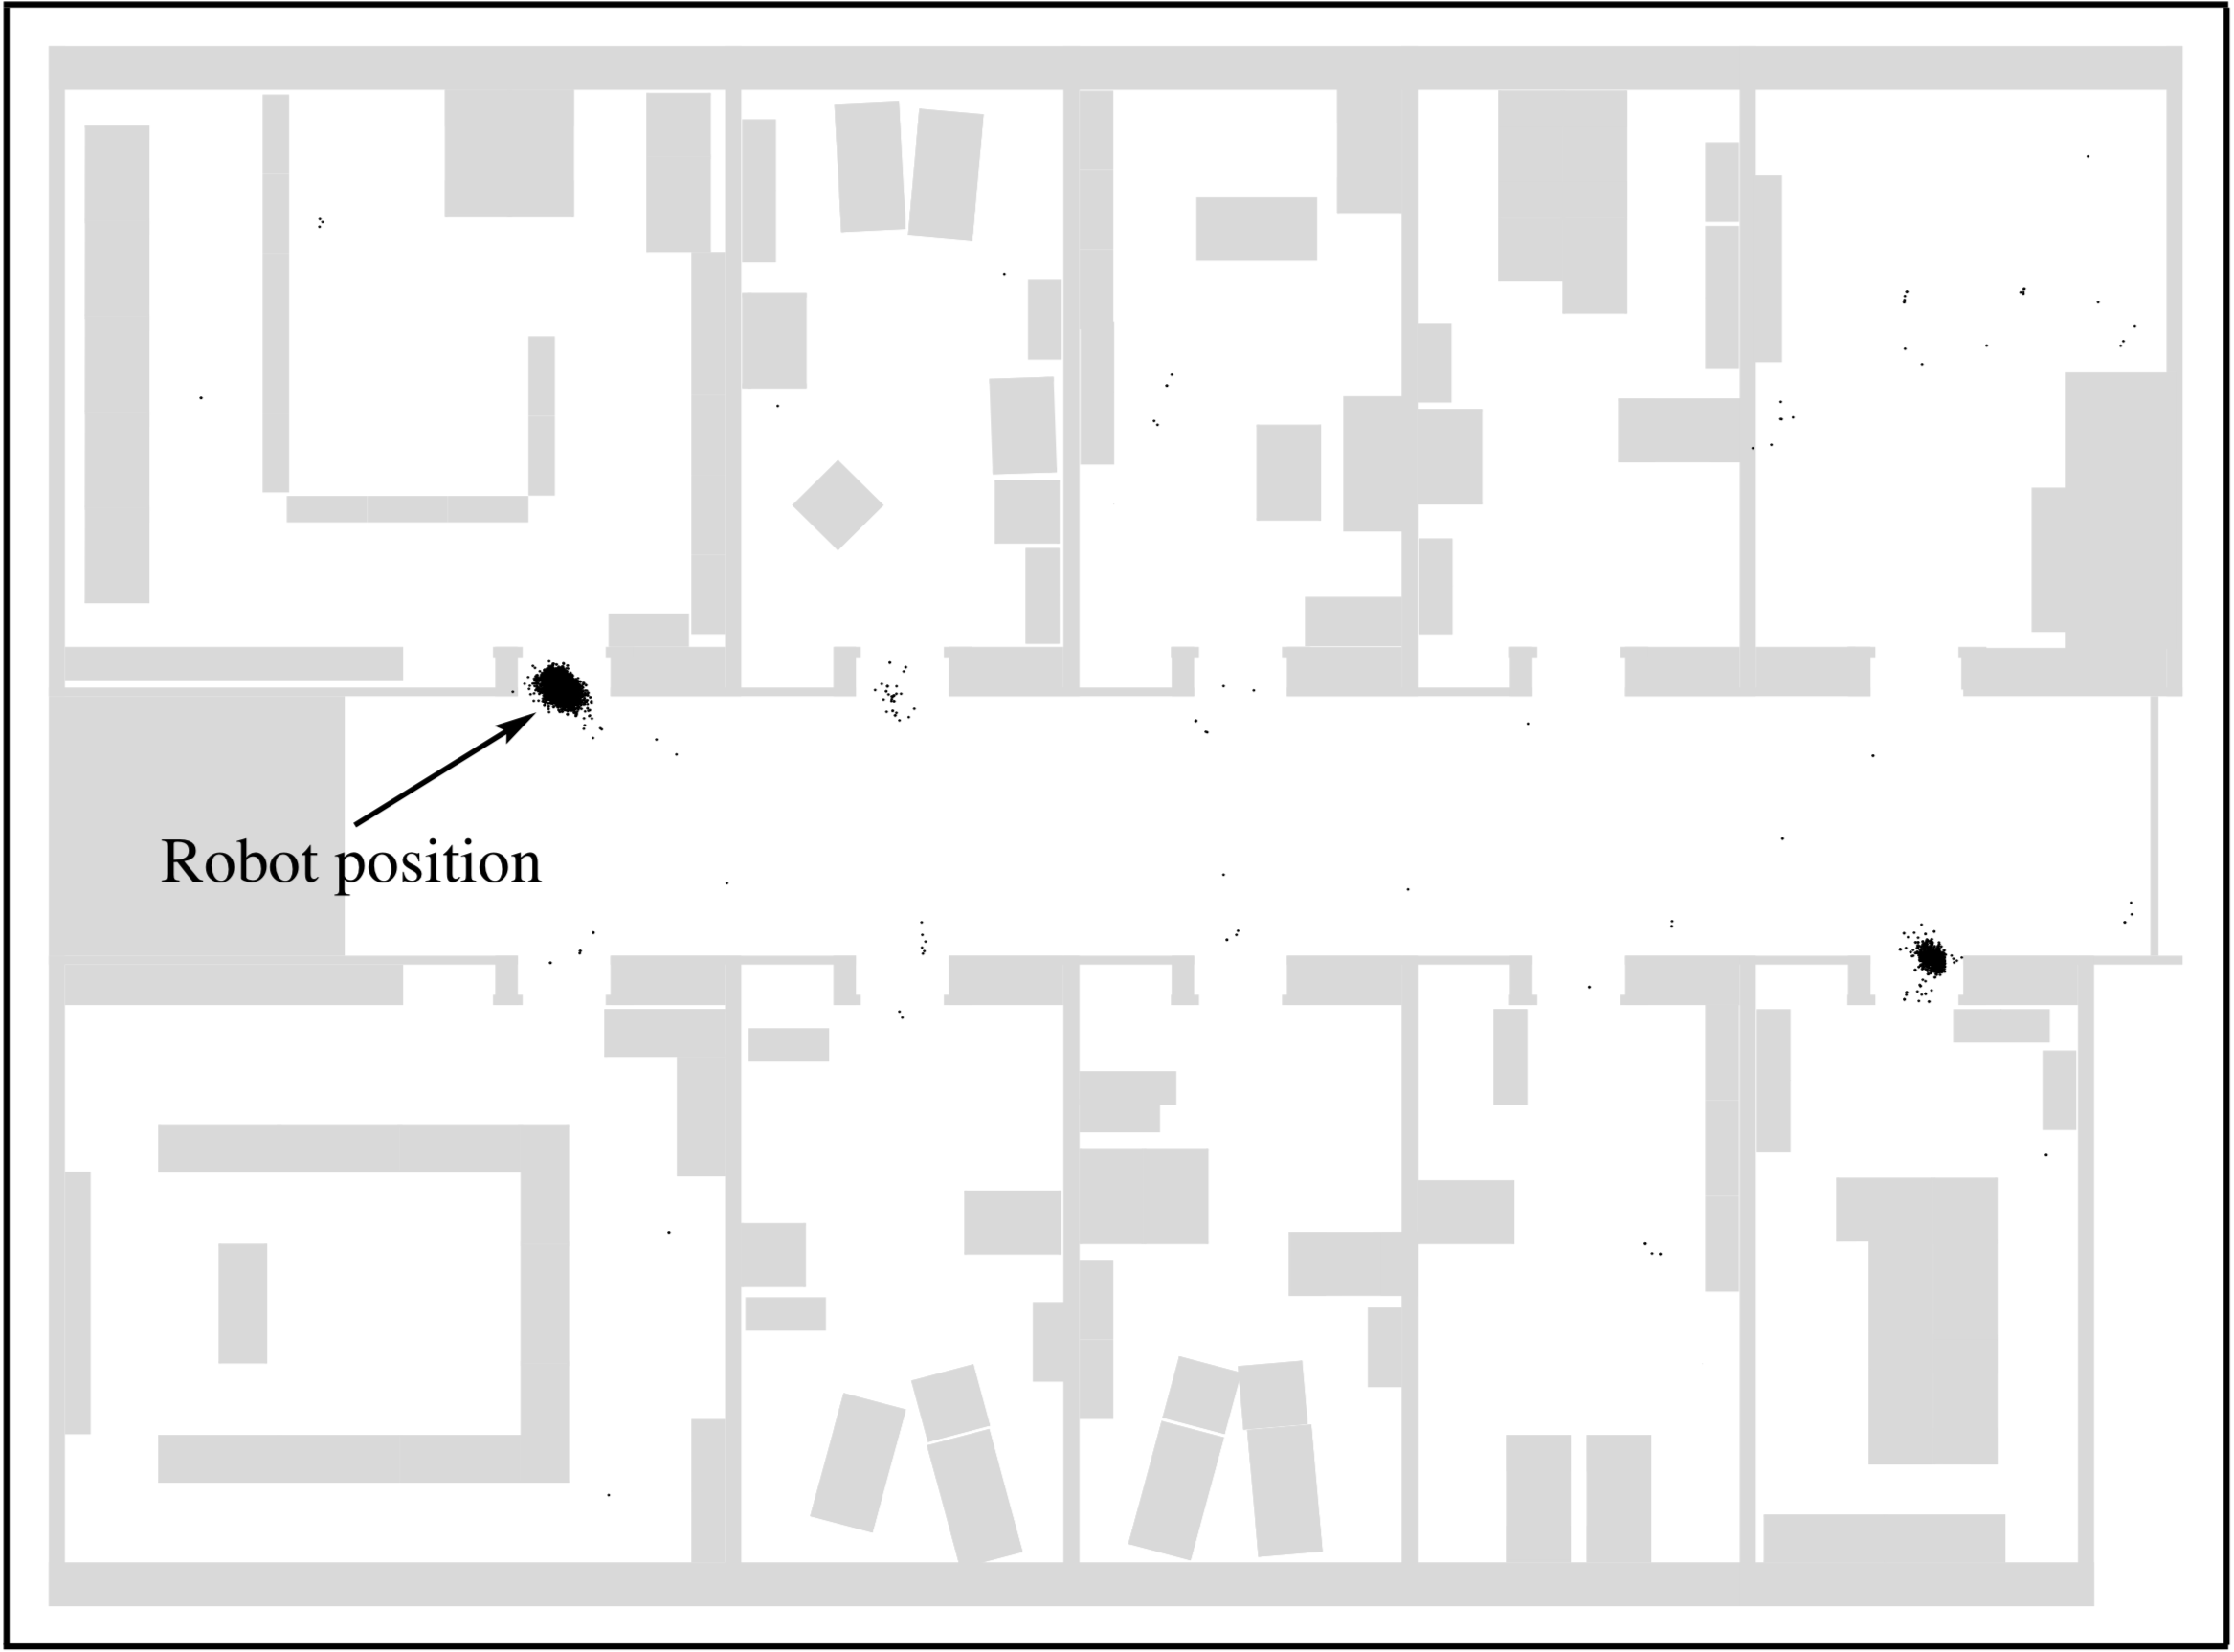
\includegraphics[width=\linewidth]{\images/chapter2/particles-2.png}
	\caption{}
  	\label{fig:ch-2:particles-2}
  \end{subfigure}
  \vspace{0.00mm}
  \begin{subfigure}[b]{0.47\linewidth}
  	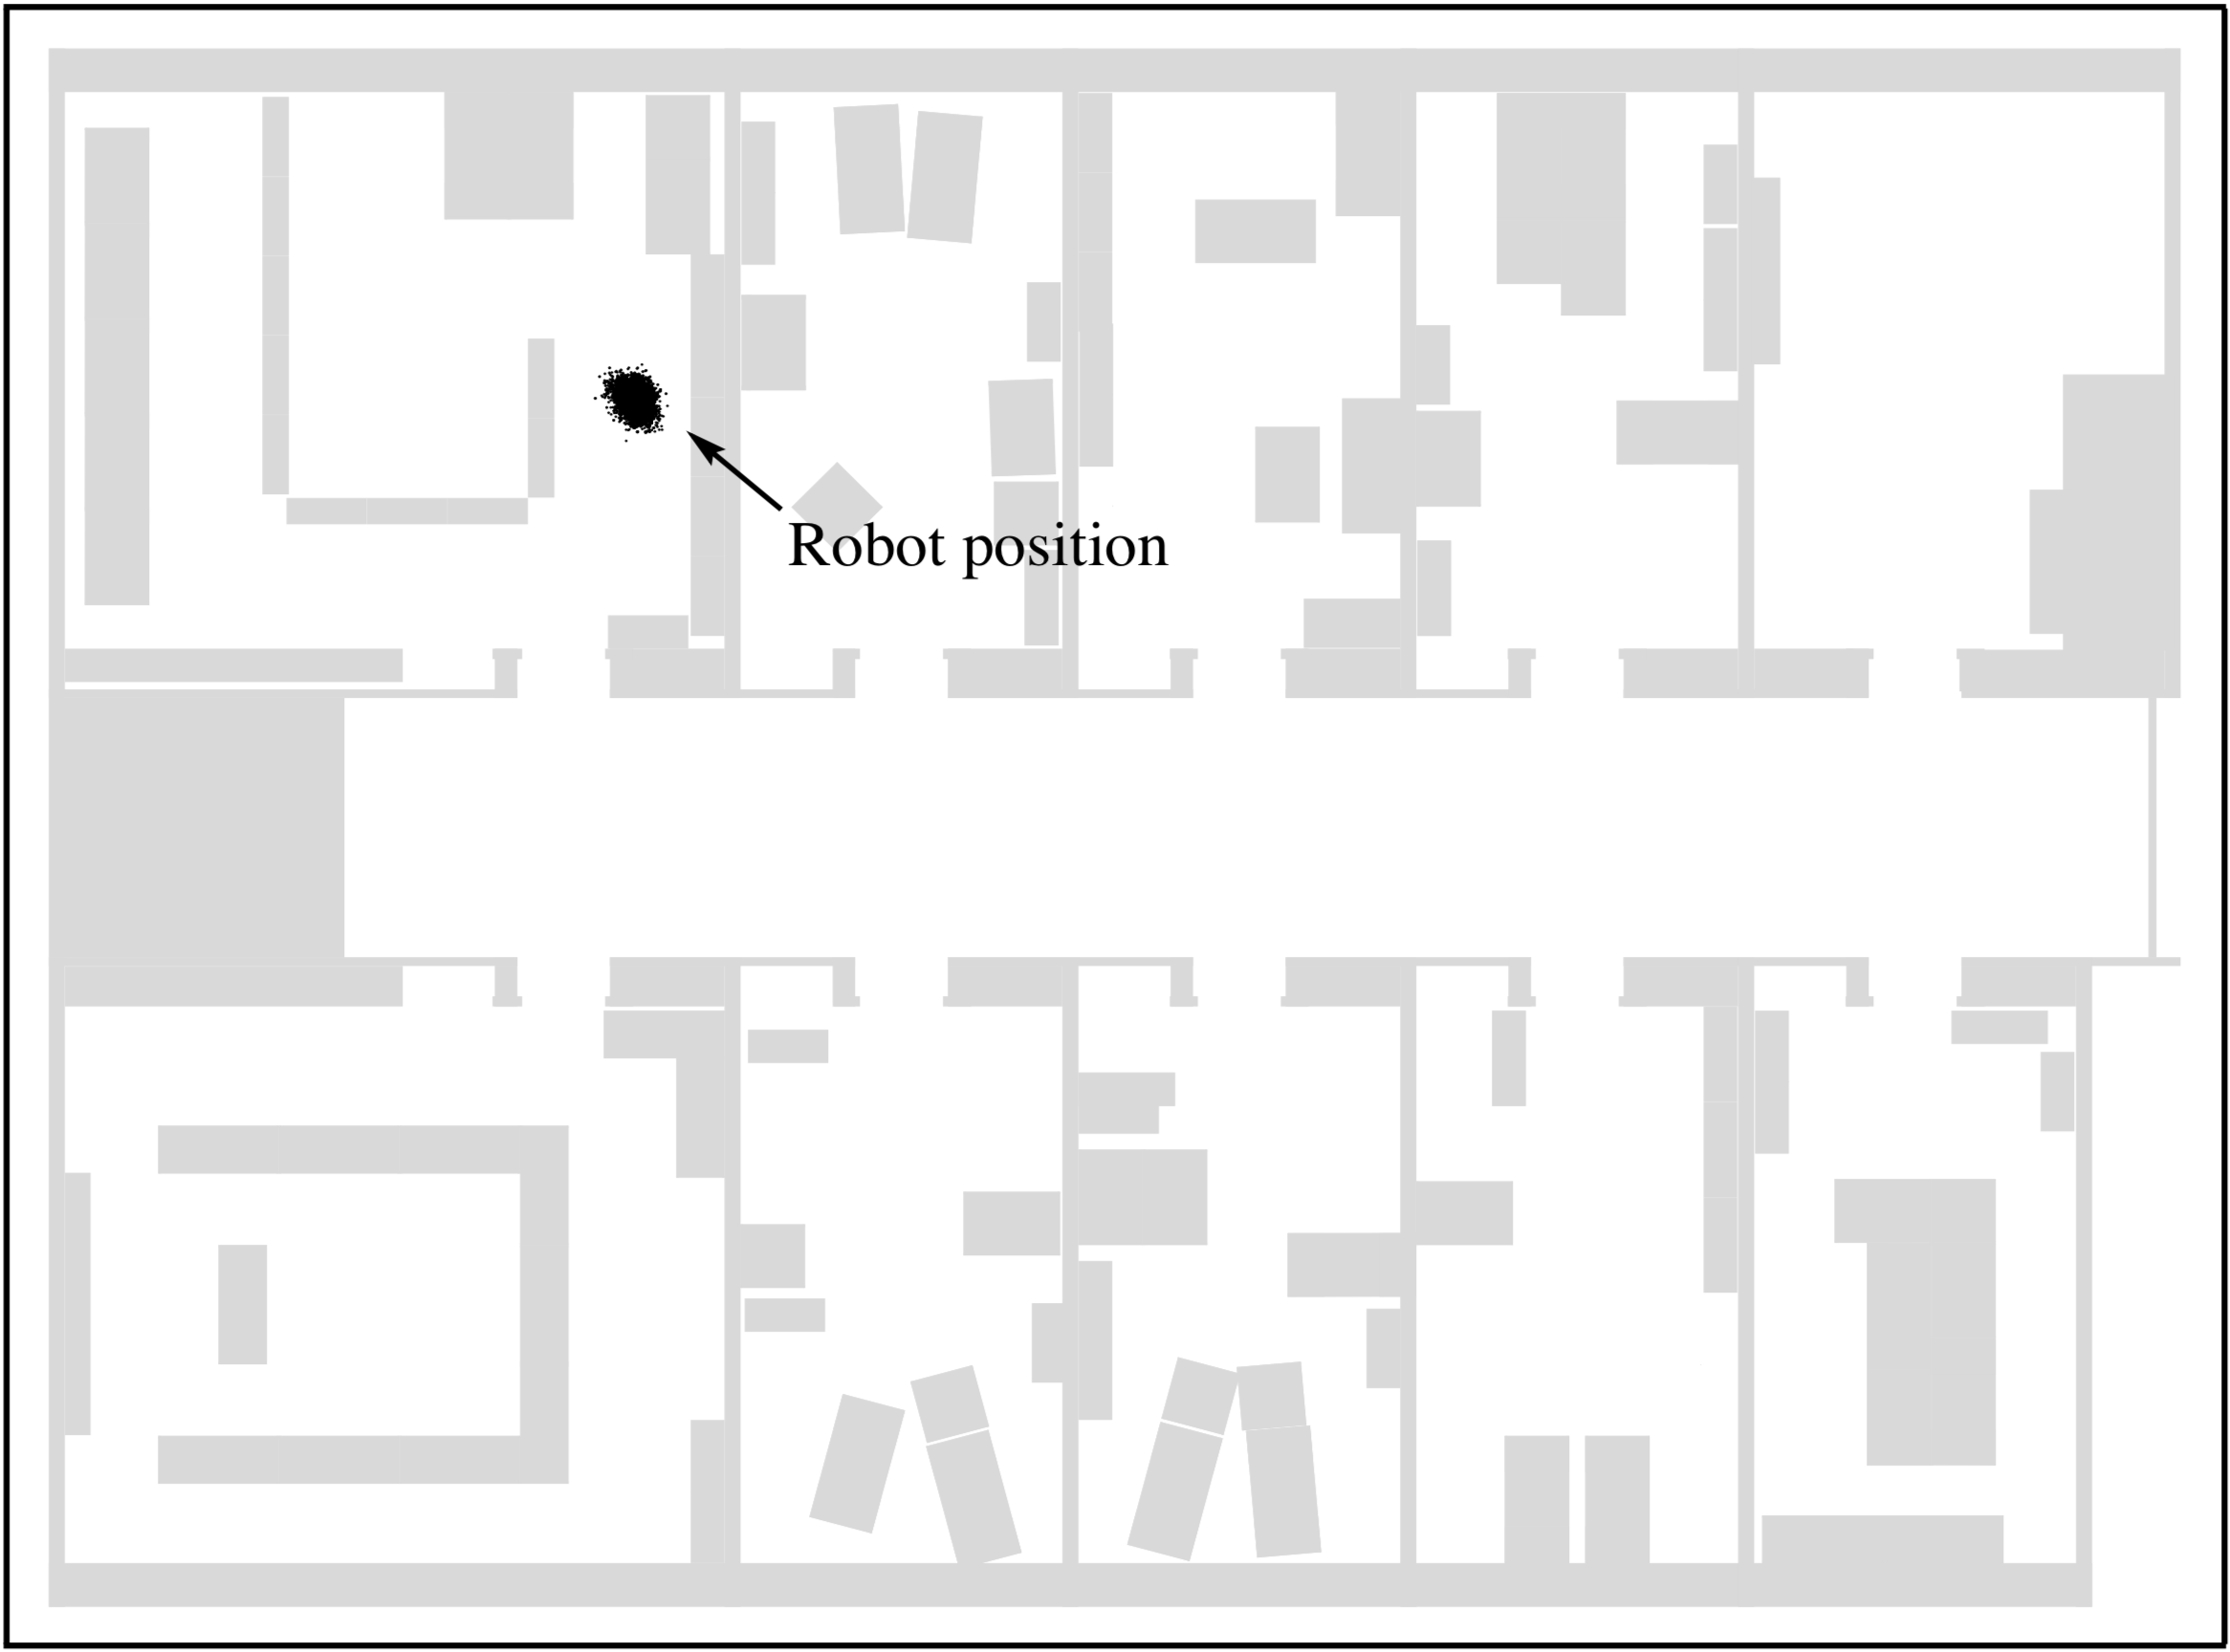
\includegraphics[width=\linewidth]{\images/chapter2/particles-3.png}
	\caption{}
  	\label{fig:ch-2:particles-3}
  \end{subfigure}
  \vspace{0.00mm}
  \caption[A robot localization example using PF.]{A robot localization example using PF. (\subref{fig:ch-2:particles-1}) The robot has a global uncertainty about its position in the map, (\subref{fig:ch-2:particles-2}) it handles some hypothesis about where it is after executing certain control actions, (\subref{fig:ch-2:particles-3}) it is quite sure where it is in the environment.}
  \source{Particles Filters in Robotics\cite{Thrun:particle-filter-robotics}.}
  \label{fig:ch-2:particles-ex}
\end{figure}

As claimed by Thrun, one drawback of PF is that the performance of the algorithm highly depends on the environment dimension, that is, higher the dimension, worst its performance is. For instance, simultaneous localization and mapping problem (SLAM) is a clear example in which the robot does not have a previous built map, deals with a high-dimensional environment and does not have any information about its initial position. Consequently, SLAM cannot be resolved using conventional MCL algorithms due to the absence of an initial map. Doucet et al. find a solution to this problem with a variation of PF called Rao-Blackwellised Particle Filter resolving the problem efficiently up until 100000 dimensions\cite{Doucet:2000:RPF:2073946.2073968}. Montemerlo et al. proposed FastSLAM, an algorithm that recursively estimates the full posterior distribution over robot pose and landmark locations\cite{Montemerlo02a} and it is one of the most robust algorithms for mapping in-door environments\cite{Thrun:particle-filter-robotics}.


\section{Related Work}

Models nowadays claim for conditional branching, loops and recursion over trees\cite{inproceedings:ML-ProgrammingLang}. That is why the idea of Differentiable Programming (DP) has emerged recently in the machine learning community, popularized by Yann LeCun\cite{LeCunn:2018}. DP refers to a programming model that is constructed using neural network blocks with data-dependent branches and recursion, being trainable using back propagation and gradient descent\cite{NIPS2018_8221}. For instance, the differentiable version of branching can be implemented using the Sigmoidal function, the loops can be represented through Recursive Neural Networks, arithmetic operations using the Neural Arithmetic Logic Unit, etc.\cite{Scardapane:2019}. 

Jonschkowski et al.\cite{DBLP:journals/corr/abs-1805-11122} presented the Differentiable Particle Filters (DPFs), a differentiable version of the classic particle filter algorithm with end-to-end learnable models. The recursive state prediction and correction steps are encoded in the DPFs structure which is made of a recurrent network representing the filtering loop. Even though their experiments reduces the error rates by 80\% compared to algorithmic priors, it presents the limitation of resampling as a non-differentiable operation which stops the gradient computation after a single loop iteration limiting the scope of the implementation to supervised learning.

The popularity of DP has been extended through the field of Probabilistic Robotics. Karkus et al.\cite{karkus2018particle} proposed the Particle Filter Network (PF-net), a fully differentiable system model that encodes the particle filter algorithm trained end-to-end from data. Unlike DPFs, PF-net  solves the limitation of resampling as a non-differentiable operation presenting a differentiable approximation. PF-Net is used for Visual Localization with different kind of cameras: RGB, depth, RGB-D, simulated 2D Lidar, and a Lidar-W. Their observation model receives a spatial transformation of a part of the 2D floor map, and the output of the transition model and the images of the camera. It feeds a neural network architecture composed by convolutional and fully connected neural networks obtaining the particle likelihood. It also includes semantic information on the map as labels for doos and room types to improve the localization task. They conduct experiments at various levels of uncertainty: local, semi-grobal and grobal localization using the House3D data set\cite{YiHouse3D} that contains a large collection of realistic buildings, obtaining better results compared to alternative network architechtures such as Histogram Filter (HF) networks\cite{Jonschkowski2017EndtoEndLH}, LSTM networks\cite{HochreiterLSTM}, PF, and odometry.

PF-net is used to develop further works on the domain of Probabilistic Robotics. For instance, Differentiable Mapping Networks (DMNs)\cite{DMNmapRepresentation} go one step further targeting the construction of a spatially structured view-embedding map which combined with PF-nets can be used for subsequent visual localization. DMN generates a structured latent map representation based on a set of image-pose pairs. The map representation is made up of pairs of viewpoint coordinates and learned image embeddings. This end-to-end differentiable model is evaluated in 3D simulated environments\cite{3DenvNeuralSceneRepr}\cite{Rosenbaum2018LearningMF} and in more real-world environments using the Street View dataset\cite{StreetViewMapsDS}, demonstrating strong performance in both.

Ma et al.\cite{ma2020discriminative} introduces a reinforcement learning framework for complex partial observations called Discriminative Particle Filter Reinforcement Learning (DPFRL). It uses a DPF in the neural network policy for reasoning with partial observations over time. It is composed of two main components: a discriminatively trained particle filter that tracks a latent belief, and an actor network that learns a policy given the belief. DPFRL are benchmarked using different problems in different domains. First, the Mountain Hike Task\cite{Igl2018DeepRLPOMDPs}, consisting of an agent that goes from a start to a goal position in a map that contains an irregular terrain with partial visibility showing that DPFRL learns faster compared to other models such as Deep Variational Reinforcement Learning (DVRL) and Gated Recurrent Unit (GRU)\cite{Igl2018DeepRLPOMDPs}. Second, Atari games using an introduced domain called Natural Flickering Atari Games that combine two challenges: the Flickering Atari Game, the partially observable version of the Atari games, where the observations are completely black frames half of the time and the Natural Atari Games where the black background is replaced by a sampled video stream. Results show that DPFRL outperformed in 7 out of 10 games. Finally, visual navigation using an RGB-D camera in the Habitat Environment\cite{DBLP:journals/corr/abs-1904-01201} with the Gibson dataset\cite{DBLP:journals/corr/abs-1808-10654} in which the robot navigates to a goal in previously unseen environments significantly outperforms both DVRL and GRU. 








